\section{Fourier Transformation}
\subsection{DFT, FFT}
\begin{frame}{\insertsection}
	\framesubtitle{\insertsubsection}
	\begin{itemize}
		\item DFT: Fourier-Koeffizienten $\beta_j = \sum\limits_{k=0}^{n-1} x_k e^{-2\pi i \frac{jk}{n}} \enspace ; j=0,\ldots,n-1$
		\item FFT: Voraussetzung $n = 2^\psi; \psi \in \mathbb{N}_0$ (Radix-2-FFT)
		% Wenn Voraussetzung mit gegebenen Daten nicht erreicht, hänge soviele 0 an die Daten hinten ran
		% bis die Anzahl eine Zweierpotenz ist, 0 fügen keinen Frequenzanteil bzw. keine Informationen hinzu
		\\ $\Rightarrow$ Divide-and-Conquer, berechne Fourier-Koeffizienten \\ \hskip 1.35em in $2$ Hälften \\
		Sei $m = \frac{n}{2}; \enspace \varepsilon_\psi = e^{-\frac{2\pi i}{2^\psi}}$ \newline
		\small{$\beta_{2\kappa} = \sum\limits_{k=0}^{m-1} (x_k+x_{k+m})\varepsilon_{\psi-1}^{\kappa k} ; \enspace \kappa = 0,\ldots,m-1$}
		\small{$\beta_{2\kappa+1} = \sum\limits_{k=0}^{m-1} ((x_k-x_{k+m})\varepsilon_{\psi}^{\kappa k})\varepsilon_{\psi-1}^{\kappa k}$}
		%\\ $\Rightarrow$ u.a. $\varepsilon_{\psi-1}^{\kappa k}$ kommt in beiden Gleichungen vor \vspace{0.5em}
		\vspace{0.5em}
		\\ $\Rightarrow$ insgesamt halbiert sich der Rechenaufwand
	\end{itemize}
\end{frame}

\begin{frame}{\insertsection}
	\framesubtitle{\insertsubsection}
	\begin{itemize}
		\item DFT ist konjugiert symmetrisch\myfootcite{conjugateSymmetry}, \\ wenn Datenwerte $x_j \in \mathbb{R}$ %sind
		\begin{align*}
			\beta_{n-j} & = \sum\limits_{k=0}^{n-1} x_k \cdot e^{-2\pi i \frac{(N-j)k}{n}} =  \sum\limits_{k=0}^{n-1} x_k \cdot \overline{e^{-2\pi i \frac{jk}{n}}} \\
			& =  \sum\limits_{k=0}^{n-1} \overline{x_k \cdot e^{-2\pi i \frac{jk}{n}}} = \overline{\beta_j}
			% funktioniert nur wenn x_j reell damit Im(x_j) = 0 ist und somit x_j = Conj(x_j)
		\end{align*}
		\\ $\Rightarrow$ es reicht DFT von Datenwerten $x_j$ \\ \hskip 1.35em mit $j \in [0,n/2]$ zu berechnen
	\end{itemize}
\end{frame}



\subsection{Performance}
\begin{frame}{\insertsection}
	\framesubtitle{\insertsubsection}

	\begin{columns}[T] % align columns{\tiny }
	\begin{column}{0.6\textwidth}
		\begin{figure}
			\centering
			\includegraphics[scale=0.3]{images/Runtime\_DFT\_FFT\_1e6.png}
			%\caption{\centering Laufzeitverhalten von \\ DFT, FFT}
		\end{figure}
		\begin{itemize}
			\item Jede Iteration berechnet $e^{-2\pi i \frac{jk}{n}}$
			\\ $\rightarrow$ Benchmark\myfootcite{Benchmark-std::exp}: ca. $\SI{5}{\nano\second}$
		\end{itemize}
	\end{column}
	\hfill
	\begin{column}{0.48\textwidth}
		\begin{itemize}
			\vspace{1em}
			\item[] Für $n=10^6$, also eine WAV Datei mit $10^6$ Datenwerten ($\SI{2}{\mega\byte}$) gilt:
			\item DFT $ \approx 10^{12}$ Iterationen
			\\ $\Rightarrow$ Berechnung dauert ca. $10^{12} \cdot \SI{5}{\nano\second} = \SI{5000}{\second} \newline \approx \SI{83}{\minute}$ 
			\item FFT $ \approx 10^{7}$ Iterationen
			\\ $\Rightarrow$ Berechnung dauert ca. $10^{7} \cdot \SI{5}{\nano\second} = \SI{0.05}{\second}$
		\end{itemize}
	\end{column}
	\end{columns}
\end{frame}



\subsection{IDFT}
\begin{frame}{\insertsection}
	\framesubtitle{\insertsubsection}
	
	\begin{itemize}
		\item im Grunde ist IDFT nur eine DFT mit Normalisierungsfaktor
		\\ $x_j = \frac{1}{n} \sum\limits_{k=0}^{n-1} \beta_k e^{2\pi i \frac{jk}{n}} \enspace ; j=0,\ldots,n-1$ \vspace{0.5em}
		\item Matrix-Schreibweise: \\ %\vspace{0.25em}
		$\begin{bmatrix}
			\omega^{jk}
		\end{bmatrix}
		\begin{bmatrix}
			\omega^{jk}
		\end{bmatrix}^\dag
		= n \cdot E_n
		\enspace; j,k=0,\ldots,n-1$
		\item[] mit $\omega = e^{-2\pi i \frac{1}{n}}$
		%\vspace{0.5em}
		\item auch IFFT existiert um IDFT zu berechnen
	\end{itemize}
\end{frame}


\subsection{Konvergenzverhalten, Fehleranalyse}
\begin{frame}{\insertsection}
	\framesubtitle{\insertsubsection}
	\begin{itemize}
		\vspace{1em}
		\item Fourier-Reihe konvergiert punktweise\myfootcite{KonvergenzFourierReihe},
		\\ gleichmäßige Konvergenz in kompakten Intervallen in denen $f(t)$ stetig ist
		\item Gibbssches Phänomen: Überschwingung an Unstetigkeitsstellen um mind. $9\%$ bei abgebrochener Fourier-Reihe
	\end{itemize}
	\begin{figure}
		\centering
		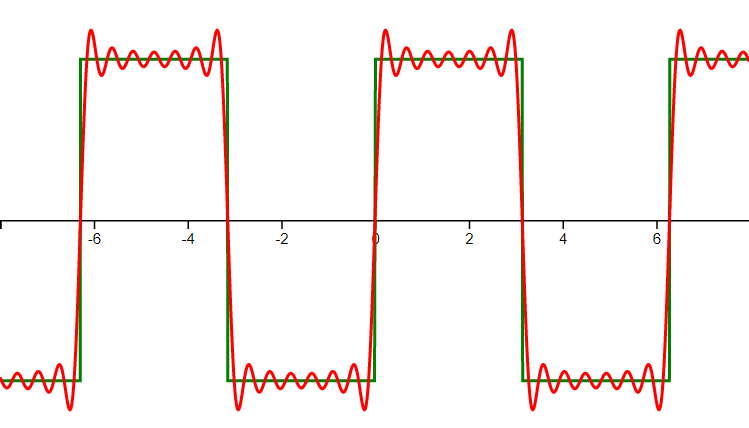
\includegraphics[scale=0.15]{images/gibbs.png}
		\caption*{\centering Gibbsches Phänomen, \\ \href{https://resources.altium.com/de/p/how-gibbs-phenomenon-produces-measurement-artifacts}{https://resources.altium.com/de/p/how-gibbs-phenomenon-produces-measurement-artifacts}}
	\end{figure}
\end{frame}

\begin{frame}{\insertsection}
	\framesubtitle{\insertsubsection}
	\begin{itemize}
		\item DFT als Matrix ist eine Vandermonde-Matrix: \\ \vspace{0.5em}
		$\begin{bmatrix}
			1 & 1 & 1 & \cdots & 1 \\
			1 & \omega & \omega^2 & \cdots & \omega^{n-1} \\
			1 & \omega^2 & (\omega^2)^2 & \cdots & (\omega^2)^{n-1} \\
			\vdots & \vdots & \vdots & \ddots & \vdots \\
			1 & \omega^{n-1} & (\omega^{n-1})^2 & \cdots & (\omega^{n-1})^{n-1} \\
		\end{bmatrix} $ \vspace{0.5em}
		\item Vandermonde-Matrizen sind grundsätzlich schlecht konditioniert,
		%$det = \prod\limits_{0 \le i < j \le n} (x_j - x_i)$
		Ausname: DFT ist gut konditioniert\myfootcite{VandermondeCondition}
	\end{itemize}
\end{frame}


\subsection{Leck-Effekt, Fensterfunktionen}
\begin{frame}{\insertsection}
	\framesubtitle{\insertsubsection}
	
	\begin{itemize}
		\item Anzahl der Datenpunkte eines zeitdiskreten Signals ist kein ganzzahliges Vielfaches der Periodendauer
		% sehr wahrscheinlich dass der Fall eintritt
		\item DFT gibt Frequenzanteile an, die im unendlich langen Signal nicht vorkämen
		\item Leck-Effekt (spectral leakage) tritt auf, weil das Signal nur endlich lange beobachtet werden kann
	\end{itemize}
	
	\begin{columns}[T] % align columns{\tiny }
		\begin{column}{0.48\textwidth}
			\begin{figure}
				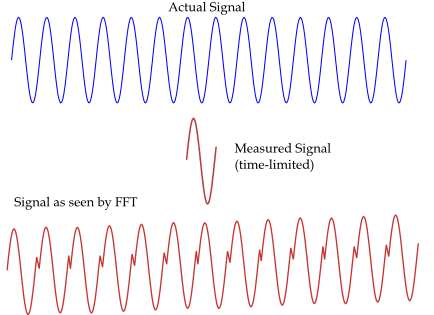
\includegraphics[scale=0.25]{images/spectralLeakage.png}
				\caption*{\centering Zustandekommen des Leck-Effekts, \href{https://www.gaussianwaves.com/2011/01/fft-and-spectral-leakage-2/}{\tiny https://www.gaussianwaves.com/2011/01/fft-and-spectral-leakage-2/}}
			\end{figure}
		\end{column}
		\hfill
		\begin{column}{0.5\textwidth}
			\begin{figure}
				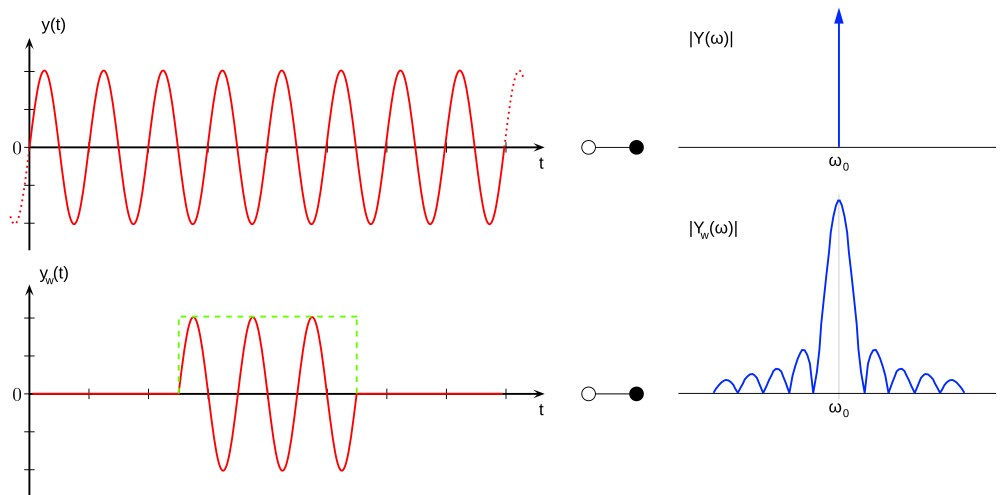
\includegraphics[scale=0.185]{images/spectralLeakage-WindowFunction.png}
				\caption*{\centering implizite Anwendung eines Rechteck-Fensters, \href{https://de.wikipedia.org/wiki/Leck-Effekt}{\tiny https://de.wikipedia.org/wiki/Leck-Effekt}}
			\end{figure}
		\end{column}
	\end{columns}
\end{frame}

\begin{frame}{\insertsection}
	\framesubtitle{\insertsubsection}
	
	\begin{itemize}
		\vspace{1em}
		\item Leck-Effekt lässt sich nicht komplett vermeiden
		\item Auswirkung aber reduzierbar durch Fensterfunktionen
		\item Fensterfunktion wird vor der DFT Operation auf das Signal angewendet, sodass das Signal
				  künstlich periodisiert wird
				  % wenn man kein Fenster verwendet wird implizit das Rechteck-Fenster (Daten*1) angewendet,
				  % weil die Daten nur endlich lang sind
				  % Faltungssatz: Multiplikation im Zeitbereich ist Faltung der Fourier Transformierten und andersherum
				  % => Frequenzspektrum ist die Faltung aus DFT(Daten), DFT(Rechteck)
				  % wobei DFT(Rechteck) die Sinc-Funktion ist und diese hat Ripples
	\end{itemize}
	\begin{figure}
		\centering
		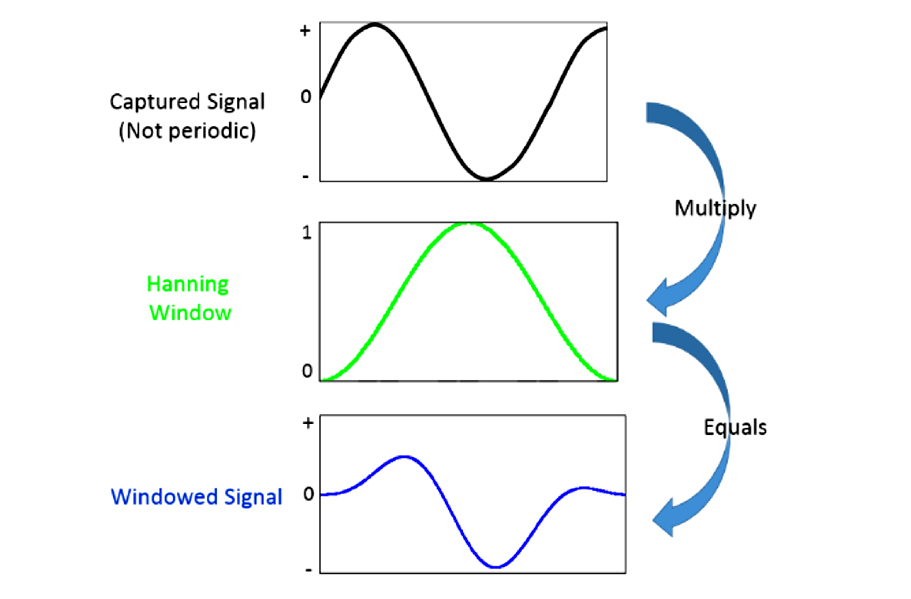
\includegraphics[scale=0.4]{images/appliedWindowFunction2.jpg}
		\caption*{\centering Anwendung des Von-Hann-Fensters,\\ \href{https://www.modalshop.com/rental/learn/basics/how-to-choose-fft-window}{\tiny https://www.modalshop.com/rental/learn/basics/how-to-choose-fft-window}}
	\end{figure}
\end{frame}














 
